145. \begin{figure}[ht!]
\center{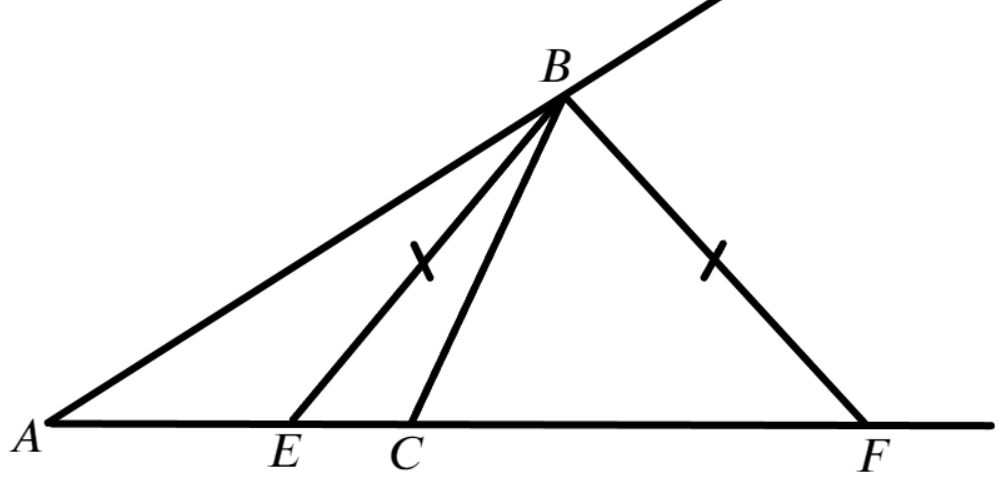
\includegraphics[scale=0.35]{g7-145.png}}
\end{figure}\\
Пусть $\angle B=\beta,$ тогда $\angle EBC=\cfrac{\beta}{2},\ \angle CBF=\cfrac{180^\circ-\beta}{2},\ \angle EBF=\cfrac{\beta}{2}+\cfrac{180^\circ-\beta}{2}=90^\circ.$ Значит, в равнобедренном треугольнике $EBF$ углы $BEF$ и $BFE$ равны по $\cfrac{180^\circ-90^\circ}{2}=45^\circ.$ Тогда из треугольника $ABF$ получим $\angle A=180^\circ-\beta-\cfrac{180^\circ-\beta}{2}-45^\circ=45^\circ-\cfrac{\beta}{2},$ а из треугольника $BEC$ --- $\angle C=180^\circ-\cfrac{\beta}{2}-45^\circ=135^\circ-\cfrac{\beta}{2}.$ Таким образом, $\angle C-\angle A=135^\circ-\cfrac{\beta}{2} -\left(45^\circ-\cfrac{\beta}{2}\right)=90^\circ.$\newpage\noindent
